\chapter{Background}
\label{cha:bkg}
%Literature Review

Introduction to transformation-invariance object recognition.
What we know about the ventral visual stream.
Why use spiking neural network to model.
\section{What do we know about the brain}

\label{sec:bio}

\subsection{The Ventral Visual Pathway}
V1\\
V2\\
V4\\
IT- the main part. including IT single neuron behaviour.\\
PFC
\subsection{Untangling Object Representation}
A graphical intuition into the Problem.
\subsection{Hierarchical Abstractions}
Feed-forward, hierarchical organisation and abstraction.


\section{Spiking Neural Network}
\label{sec:pgr}
%All the literature review I can borrow from the previous report.

Dynamic recognition takes advantage of the intrinsic temporal processing of SNNs which are receiving considerable attention for  undertaking vision processing.
Pattern information can be encoded in the delays between the pre- and post-synaptic spikes since the spiking neurons are capable of computing radial basis functions (RBFs)~\cite{hopfield1995pattern}.
Spatio-temporal information can also be stored in the exact firing time rather than relative delays~\cite{natschlager1998spatial}.
Maass~\cite{maass1997networks} has proved mathematically that:
1) networks of spiking neurons are computationally more powerful than the first and second generation of neural network models;
2) a concrete biologically relevant function can be computed by a single spiking neuron, replacing  hundreds of hidden units in a sigmoidal neural net;
3) any function that can be computed by a small sigmoidal neural net can also be computed by a small network of spiking neurons.
Numerous applications using SNN-based vision processing have been successfully carried out in the past. 
A dual-layer SNN has been trained using Spike Time Dependent Plasticity (STDP) and employed for character recognition~\cite{gupta2007character}. 
Lee et al.~\cite{6467270} have implemented direction selective filters in real time using spiking neurons, considered as a convolution layer in the model of a so called CNN~\cite{camunas2012event}. 
Different features, such as Gabor filter features (scale, orientation and frequency) and shape can be modelled as layers of feature maps. 
The similar behaviours have been found in the primary visual cortex (V1) in the visual pathway~\cite{rehn2007network} as the foundation for higher level visual process e.g. object recognition.
Rank order coding, as an alternative to conventional rate-based coding, treats the first spike as the most important and has been successfully applied to an orientation detection training process~\cite{delorme2001networks}. 
Nengo~\cite{eliasmith2011nengo} is a graphical and scripting based software package for simulating large-scale neural systems and has been used to build the world's largest functional brain model, Spaun~\cite{eliasmith2012large}. 
An FPGA implementation of a Nengo model for digit recognition has been reported~\cite{naylor2013managing}. 
Deep Belief Networks (DBNs), the 4th generation of artificial neural network, have shown great success in solving classification problems. 
Recent study~\cite{o2013real} in this area has mapped an offline-trained DBN onto an efficient event-driven spiking neural network for digit recognition tasks with resounding success.

%Section~\ref{sec:np} of this paper presents the details of the hardware of the proposed neuromorphic system, including the silicon retina and the SpiNNaker platform.
%The neural network models are defined and tested on Matlab, and the model structures and experimental results stated in Section~\ref{sec:cnn}.
%In Section~\ref{sec:rrs}, the rate-based models are converted into spiking neurons, and real-time live recognition and recorded data experiments are carried out.
%The contribution of this work is summarised and the future directions are provided in Section~\ref{sec:cfw}.



\section{Platforms}
\label{sec:plt}
The outline of the platform is illustrated in Figure~\ref{fig:SysOverViewa}, where the hardware system is configured, controlled and monitored by the PC.
%Figure~\ref{fig:SysOverViewb} shows the combined hand posture recognition system; 
The jAER~\cite{delbruck2008frame} event-based processing software on the PC configures the retina and displays the output spikes through a USB link.
The host communicates to the SpiNNaker board via Ethernet to set up its runtime parameters and to download the neural network model off-line.
It visualises~\cite{6252490} the spiking activity of the network in real-time.
The photograph of the hardware platform, Figure~\ref{fig:SysOverViewb}, shows that the silicon retina connects to the SpiNNaker 48-node system via a Spartan-6 FPGA board~\cite{galluppi2012real}.
%, which was also applied to a sound localisation system.


\begin{figure}
\centering
	\begin{subfigure}[t]{0.6\textwidth}
		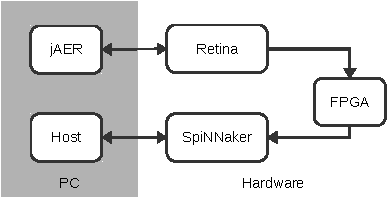
\includegraphics[width=\textwidth]{pics/outline.pdf}
	    \caption{Outline of the platform.}
	    \label{fig:SysOverViewa}
	\end{subfigure}
	\\
	\begin{subfigure}[t]{0.6\textwidth}
		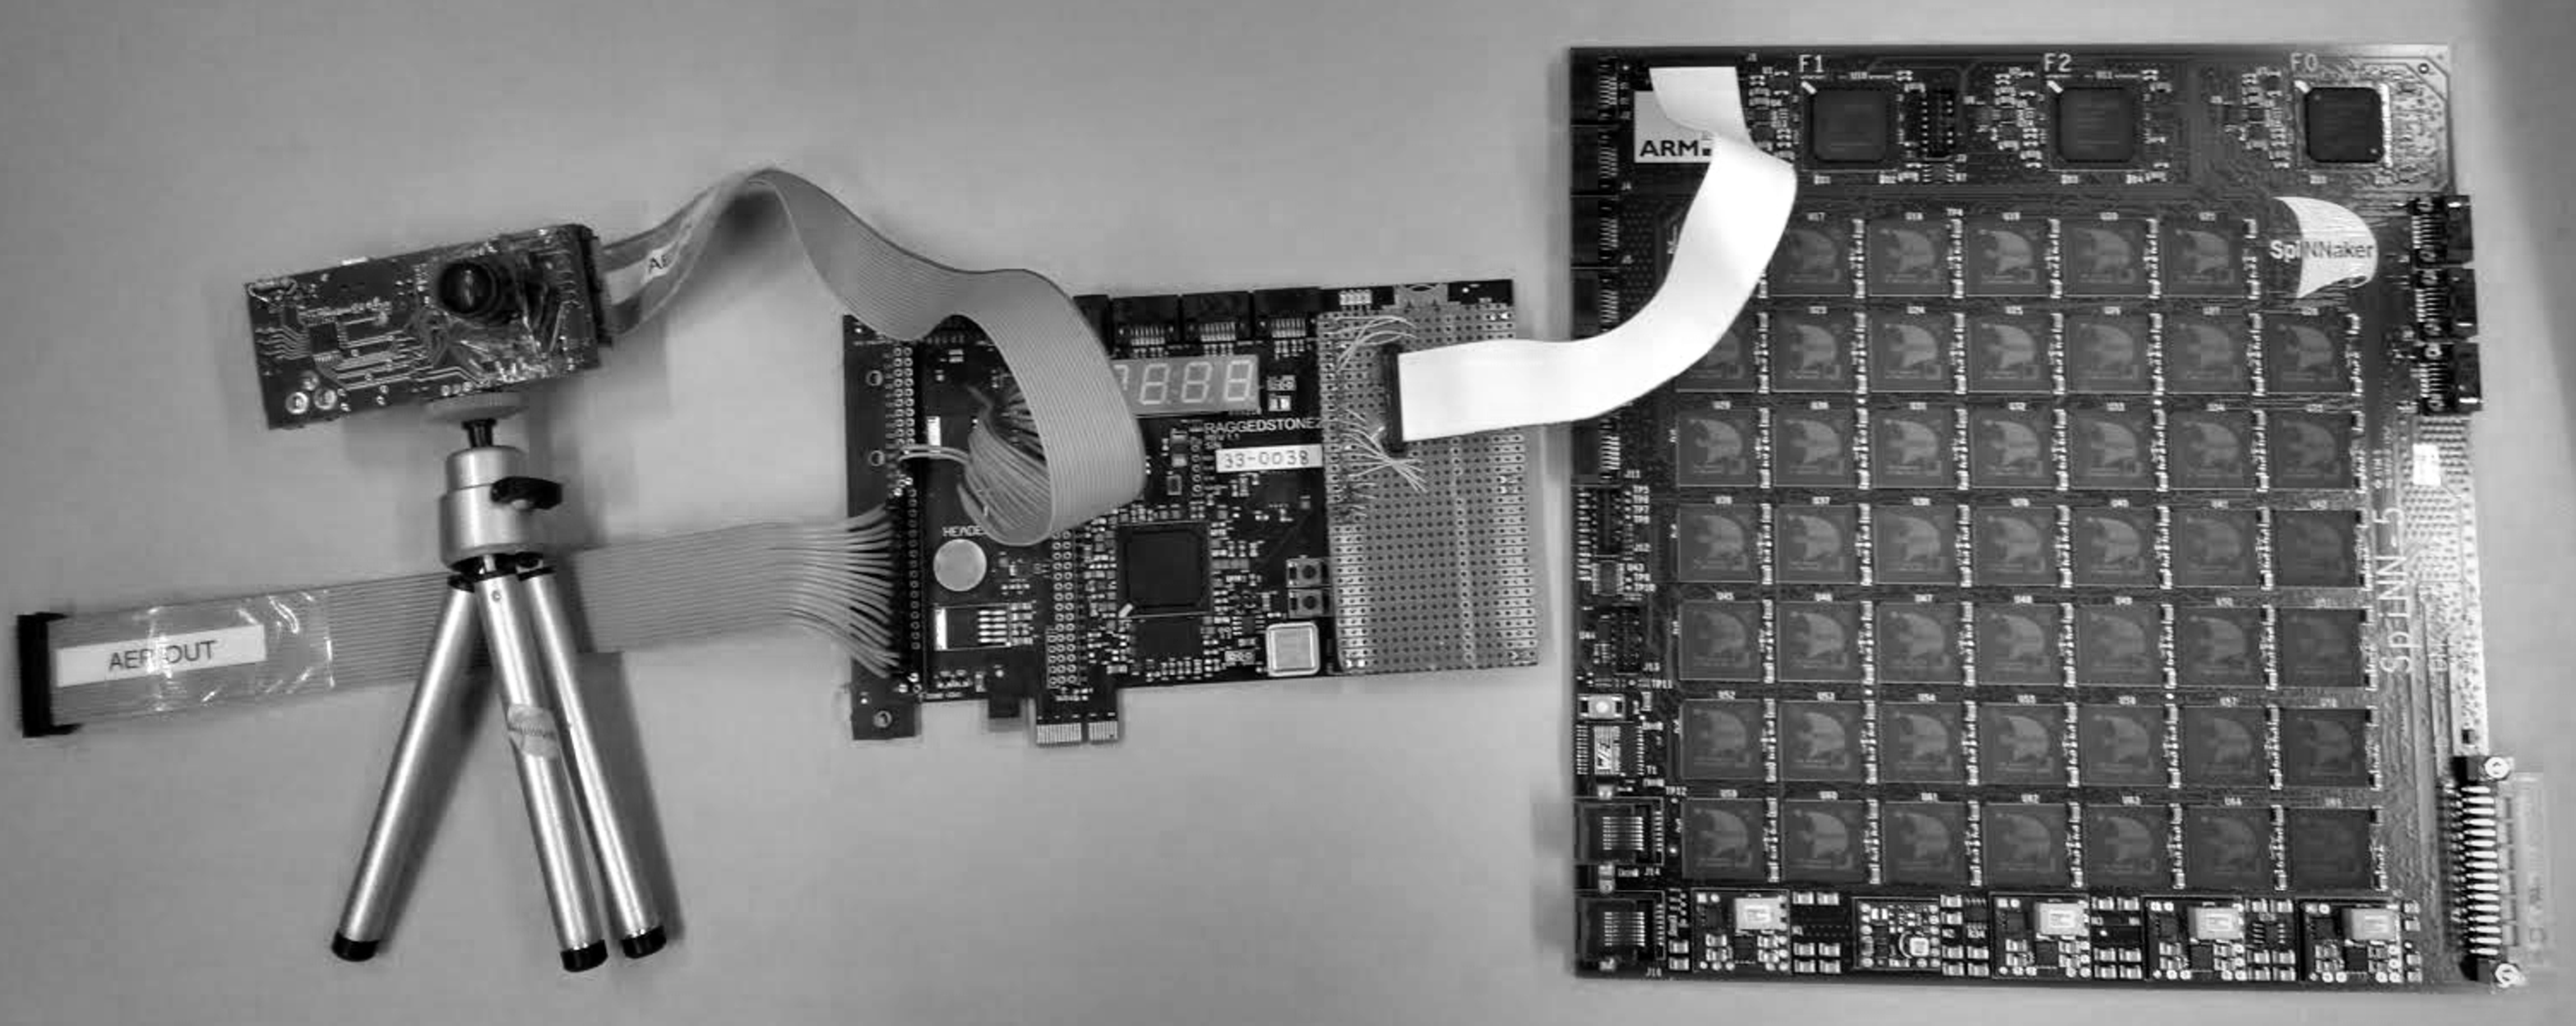
\includegraphics[width=\textwidth]{pics/outline2.pdf}	    \caption{Picture of the hardware platform. From left to right: a silicon retina, a FPGA board, and a 48-node SpiNNaker system.}
	    \label{fig:SysOverViewb}
	\end{subfigure}	

\caption{System overview of the dynamic hand posture recognition platform. 
%The silicon retina connects to the SpiNNaker system through an FPGA board. 
%Spikes from the retina are streamed to the SpiNNaker system through this Spartan-6 FPGA board.
%The jAER software configures the retina and displays its outgoing spikes through the USB connection.
%The host sets up the runtime parameters off-line and downloads the network model to the SpiNNaker system.
}
\label{fig:SysOverView}
\end{figure}


\subsection{Vision Processing Front-ends}
The visual input is captured by a DVS silicon retina, which is quite different from conventional video cameras.
Each pixel generates spikes when its change in brightness reaches a defined threshold.
Thus, instead of buffering video into frames, the activity of pixels is sent out and processed continuously with time.
The communication bandwidth is therefore optimised by sending activity only, which is encoded as pixel events using Address-Event Representation (AER~\cite{lazzaro1995multi}) protocol.
The level of activity depends on the contrast change; pixels generate spikes faster and more frequently when they are subject to more active change.
The sensor is capable of capturing very fast moving objects (e.g., up to 10 K rotations per second), which is equivalent to 100 K conventional frames per second~\cite{lenero20113}.

\subsection{SNNs Back-ends}
The SpiNNaker project's architecture mimics the human brain's biological structure and functionality. 
This offers the possibility of utilizing massive parallelism and redundancy, as the brain, to provide resilience in an environment of unreliability and failure of individual components.

In the human brain, communication between its computing elements, or neurons, is achieved by the transmission of electrical `spikes' along connecting axons. 
The biological processing of the neuron can be modelled by a digital processor and the axon connectivity can be represented by messages, or information packets, transmitted between a large number of processors which emulate the parallel operation of the billions of neurons comprising the brain.

The engineering of the SpiNNaker concept is illustrated in Figure~\ref{fig:sysdia} where the hierarchy of components can be identified. 
Each element of the toroidal interconnection mesh is a multi-core processor known as the `SpiNNaker Chip' comprising 18 processing cores. 
Each core is a complete processing sub-system with local memory.
It is connected to its local peers via a Network-on-Chip (NoC) which provides high bandwidth on-chip communication and to other SpiNNaker chips via links between them. 
In this way massive parallelism extending to thousands or millions of processors is possible.

\begin{figure}
\centering
	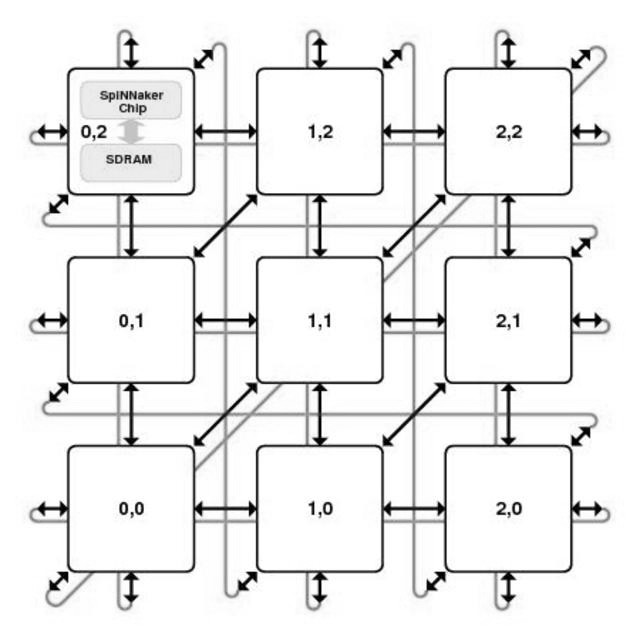
\includegraphics[width=0.8\textwidth]{pics/mesh_ctiff.jpg}
	\caption{SpiNNaker system diagram.
	Each element represents one chip with local memory.
	Every chip connects to its neighbours through the six bi-directional on-board links. }
	\label{fig:sysdia}
\end{figure}

%The knowledge content and learning ability of the brain is generally thought to be embodied in its evolvable interconnection pattern.
%This structure routes a spike generated by one neuron to others which are interconnected with it via axons and these interconnections are modified and extended as a result of learning processes.
%
%In SpiNNaker a packet router within each multi-core processor controls the neural interconnection. 
%Each transmitted packet represents a spike and simply identifies its source neuron.
%This is used by routers to identify whether a packet should be routed to a processor core, or should be routed on to one of the six adjacent chips connected to it as part of the overall SpiNNaker network.

The `103 machine' is the name given to the 48-node board which we use for the hand posture recognition system, see Figure~\ref{fig:48node}.
It has 864 ARM processor cores, typically deployed as 768 application, 48 monitor and 48 spare cores. 
%The `103 machine' requires a 12V 6A supply. 
%The control interface is via two 100Mbps Ethernet connections, one for the board management processor and the second for the SpiNNaker array. 
%There are options to use the nine on-board 3.0~Gbps high-speed serial interfaces (using SATA cables, but not necessarily the SATA protocol) for I/O; 
%this will require suitable configuration of the on-board FPGAs that provide the high-speed serial interface support. 
The boards can be connected together to form larger systems using high-speed serial interfaces. 

%\begin{figure}
%\centering
%	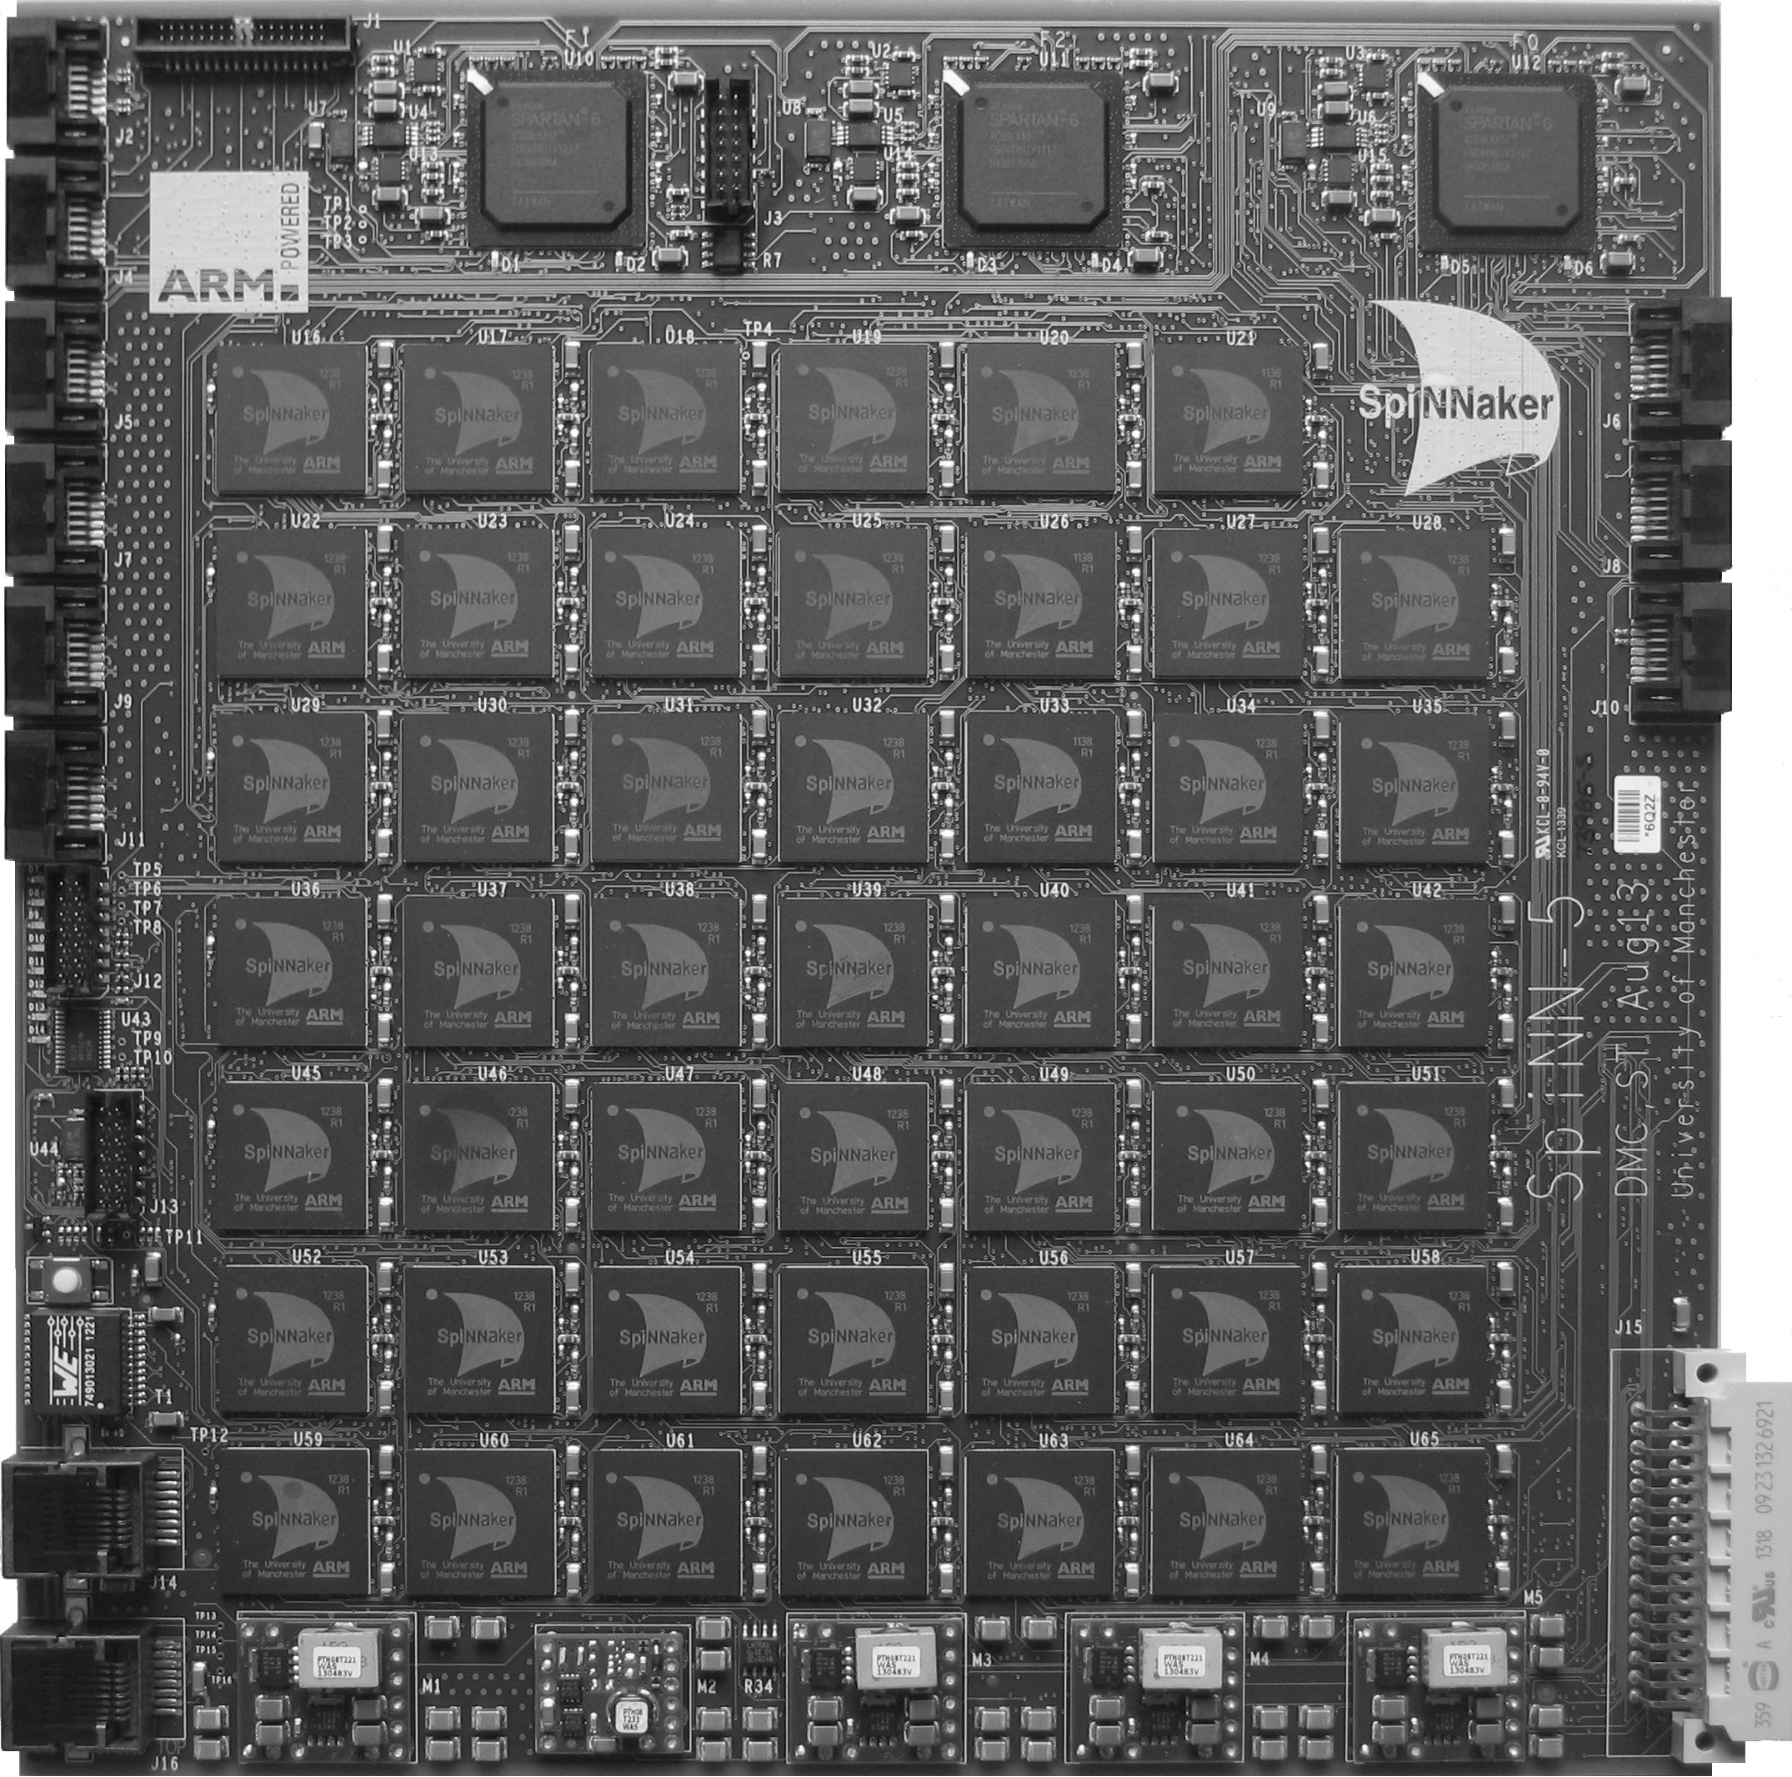
\includegraphics[width=0.6\textwidth]{pics/SpiNN5.pdf}
%	\caption{`103 Machine' PCB}
%	\label{fig:48node}
%\end{figure}

\subsection{SpiNNaker distinguishing features}
Spikes from the silicon retina are injected directly into SpiNNaker via a SPARTAN-6 FPGA board that translates them into a SpiNNaker compatible AER format~\cite{appnote8}. 

From a neural modelling point of view, interfacing the silicon retina is performed using pyNN~\cite{davison2008pynn}. 
The retina is configured as a spike source population that resides on a virtual SpiNNaker chip, to which an AER sensor's spikes are directed, thus abstracting away the hardware details from the user\cite{galluppi2012real}.
Besides the retina, we have successfully connected an AER based silicon cochlea~\cite{5537164} to SpiNNaker for a sound localisation task~\cite{6706931}.

